\subsection{Single-tagged Commit And Multi-tagged Commit}
When reviewing manual tagging, we analyze commits with different numbers of tags separately. 
The commits are divided into two groups: \textit{single-tagged} and \textit{multi-tagged}. \textit{Single-tagged} commits contain only one independent change, and \textit{multi-tagged} more than one. 

Fig. \ref{fig: cat_distribution} shows the tag-distributions of single and multi-tagged commits by commit purpose.
In the figure, black bars represent the rates when a certain commit is tagged a single category while gray bars are used to denote multi-tagged. For example, approximately 80\% commits are tagged Testing and more than 95\% of them are multi-tagged commits.
As shown in the figure, Build, Feature Add, Indentation, Refactoring, Testing arise more frequently in multi-tagged commits, indicating these tags tend to appear together with other tags. 
More than 95\% of testing commits have multiple tags, which is consistent with development practices of including the testing code along with most changes.
Documentation is more frequent in single-tagged commits, indicating that many documentation changes are added independently.
As the change of documentation is usually used to explain changed code, this may also imply that contributors often forget to add enough documentation when they accomplish a commit.
For other categories there are no apparent differences between single-tagged and multi-tagged commits.
In addition to comparing these two sets, we also study how many tags each commit has and its distribution. 
\begin{figure*}[htbp]
\centerline{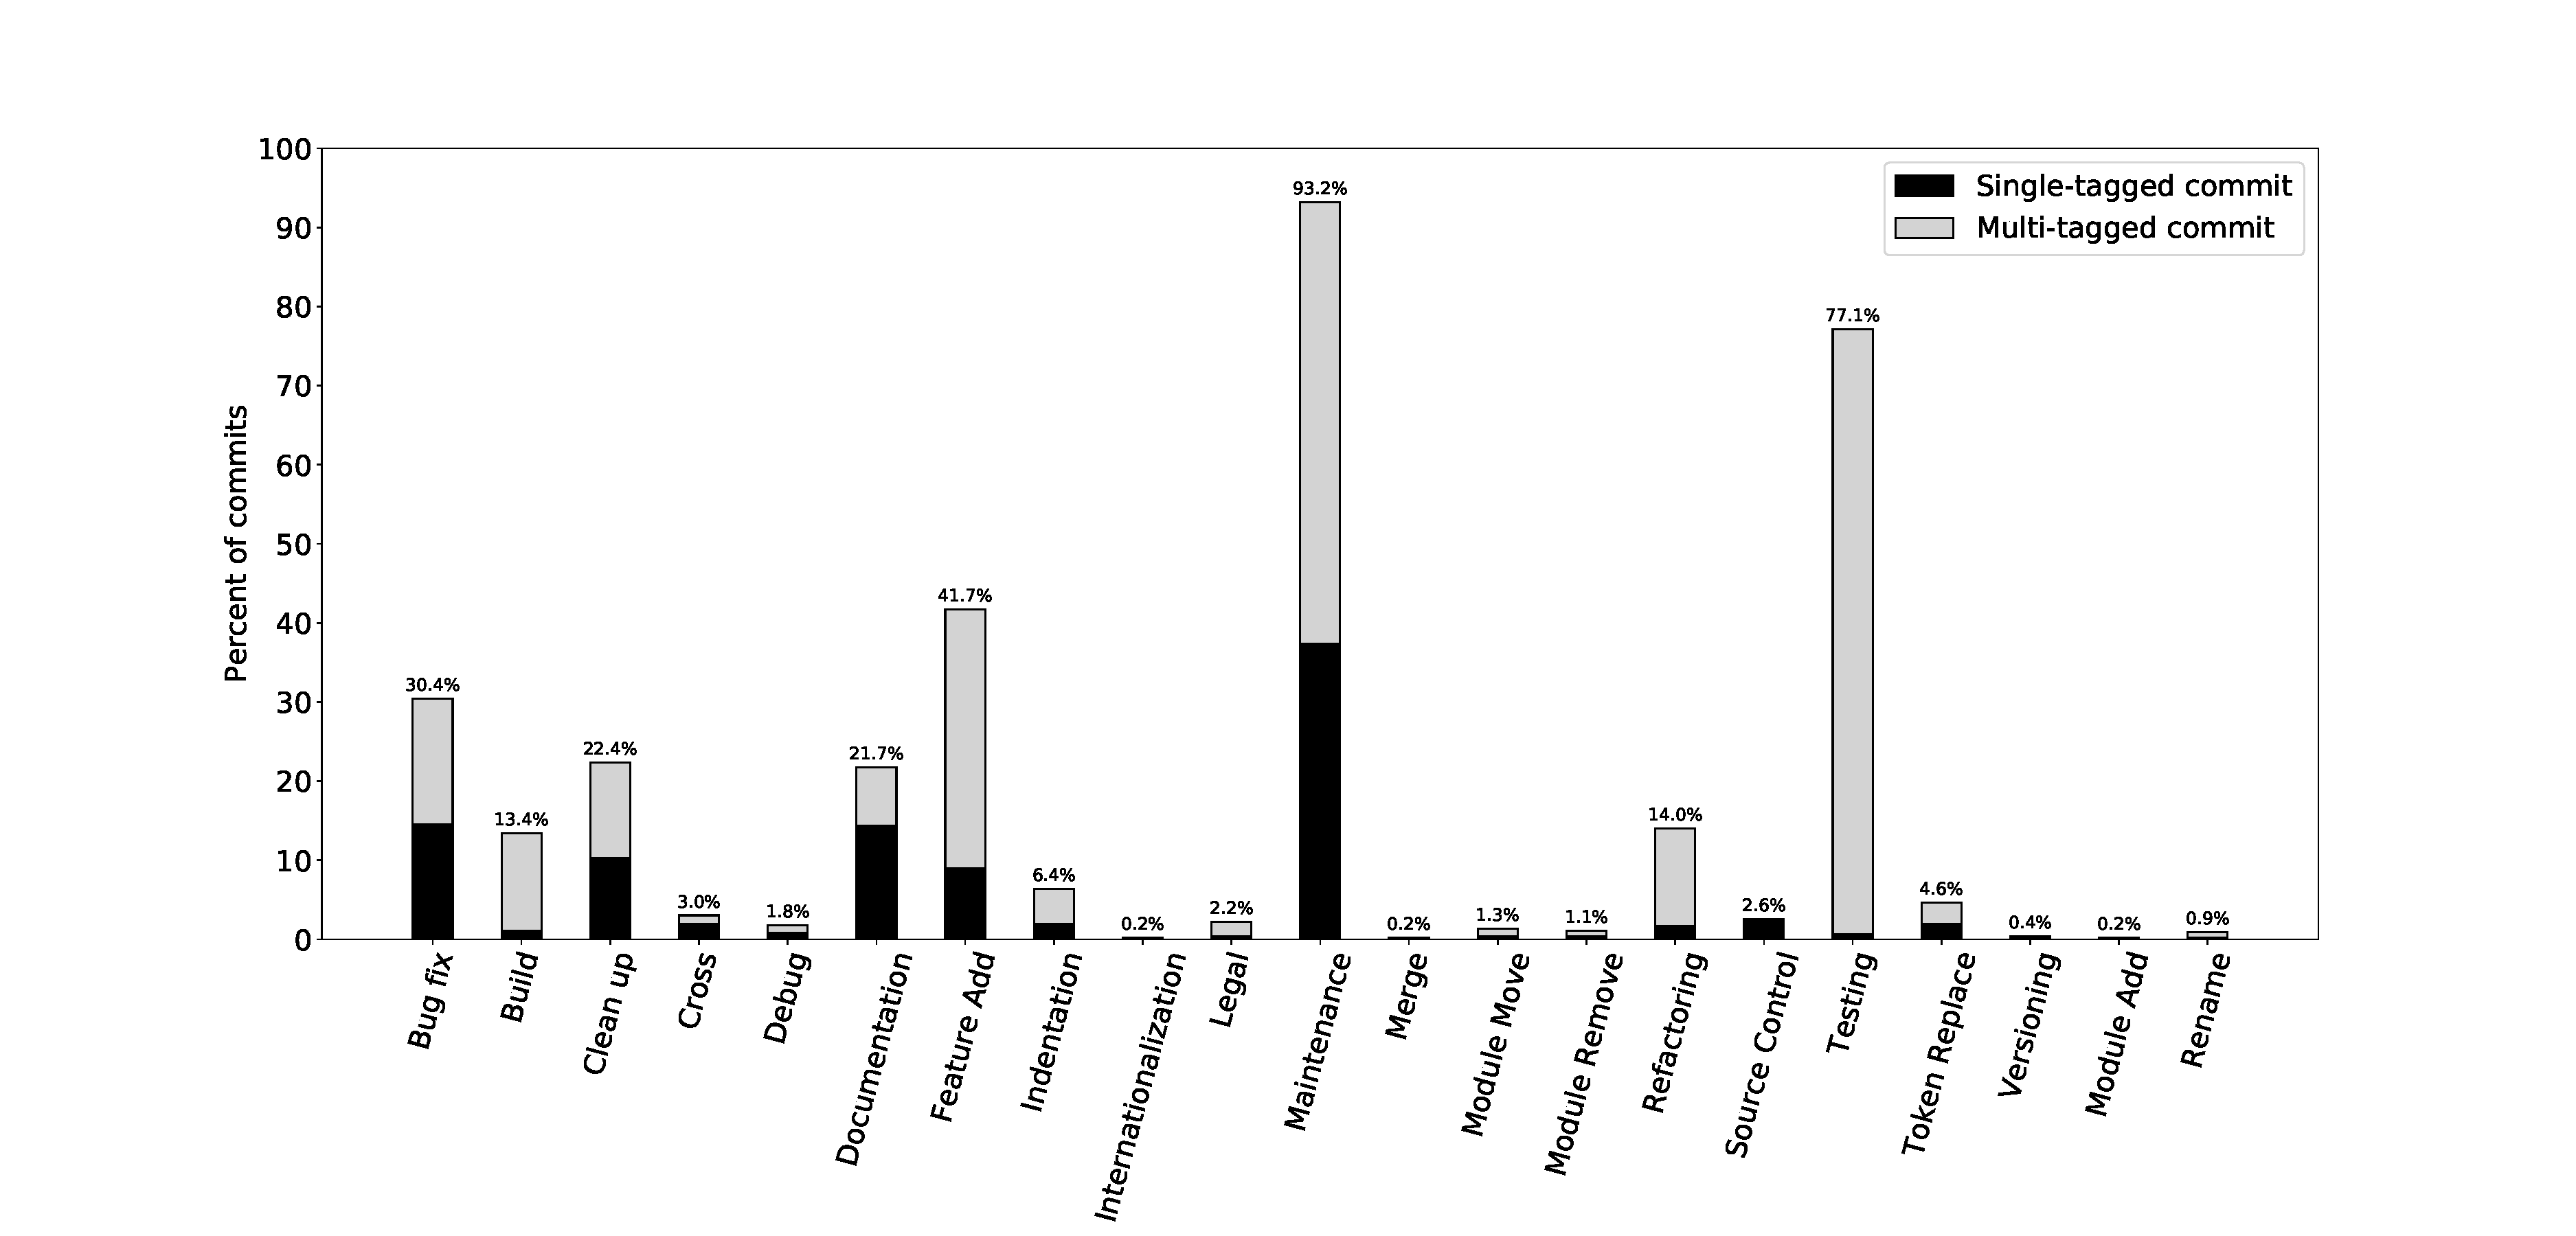
\includegraphics[scale=0.30]{figures/cat_distribution_over_s&m_commits.pdf}}
\caption{Change Type Distribution Between Single-tagged and Multi-tagged Commit}
\label{fig: cat_distribution}
\end{figure*}